\chapter{Modélisation et analyse des premières opérations de chaque pièce}
Maintenant que nous connaissons un modèle valide pour une opération ainsi que les temps nécessaires au déplacement du chariot sur l'axe vertical et horizontal, nous allons pouvoir commencer à modéliser le travail du \emph{STA} sur deux opérations.

Nous allons, dans un premier temps, effectuer une modélisation en RdP Temporels d'une commande de deux opérations suite à quoi, nous en effectuerons une analyse grâce à une version de \emph{TINA} identique que dans le chapitre \ref{chap:realisationUneOperation}. Nous utiliserons cette analyse pour déterminer les intervalles d'attentes et le meilleur ordonnancement possible pour ne pas déclencher l'alarme.

\section{Réseau de PETRI Temporels de commande de deux opérations}
A partir du modèle générique établit en \ref{sec:modelGenerique}, nous avons obtenu, pour la commande de opérations $O_1$ et $O_2$ le modèle RdP Temporels en figure \ref{fig:command2Opes}.
\begin{figure}
\centering
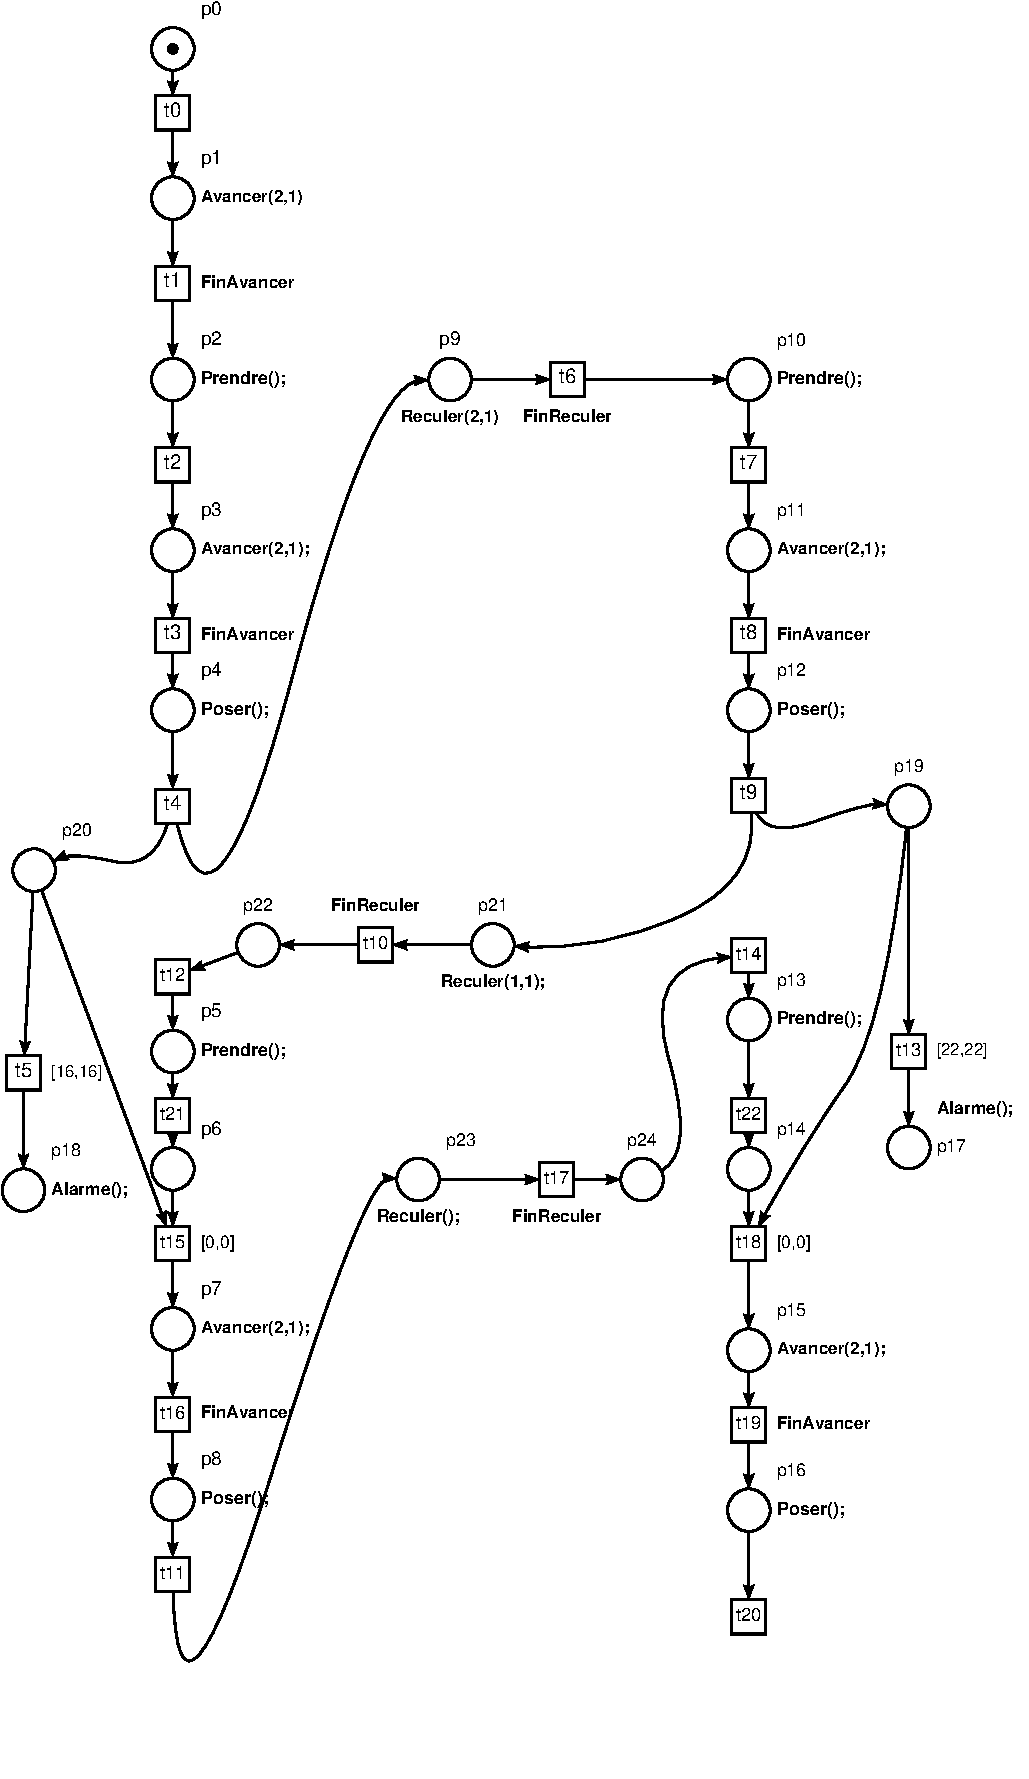
\includegraphics[height = \textheight]{./II/images/reseau_CommandeIII-2.pdf}
\caption{Réseau de PETRI Temporels pour la commande de 2 opérations}\label{fig:command2Opes}
\end{figure}

Dans ce réseau, nous pouvons identifier tout d'abord la ressemblance avec le modèle générique (en figure \ref{fig:RdPTempo_generique}) : les places $p_4$ et $p_{12}$ sont les représentations de la place $p_2$ dans le modèle générique. Elles seront donc suivi, dans les modèle Temporels que nous analyseront, d'une transition qui contient le temps des opérations \emph{Poser}. Il en va de même pour les places $p_2$, $p_{10}$, $p_{5}$ et $p_{13}$ qui contiennent l'opération \emph{Prendre}, elles seront suivi d'une transition contenant une intervalle de temps $y$.

\paragraph*{Séparation du modèle}
Nous pouvons séparer ce modèle complexe en deux ensembles de places : \begin{itemize}
\item l'ensemble $P_1 =\left\lbrace p_2,p_3,p_4,p_5,p_6,p_7,p_{20},p_{18}\right\rbrace$ est utilisé pour emmené la pièce $p2$ du bac $e2$(son bac initial) vers le bac $e5$ dans lequel elle subit l'opération $O_2$. Cet ensemble est lié avec les deux places $p_{20}$ et $p_{18}$ qui modélisent l'alarme lié à l'opération $O_2$.
\item  l'ensemble $P_2 =\left\lbrace p_{10}, p_{11}, p_{12} p_{13}, p_{14}, p_{15}, p_{16}\right\rbrace$ modélise le transport de la pièce $p1$ de $e1$(son bac initial) vers $e3$, bac dans lequel elle subit l'opération $O2$, puis du transport de $e4$ vers $e6$ (Pour prévoir les prochains RdP). L'alarme de l'opération est enclenchée par la place $p_{17}$, qui est lié au reste de l'ensemble $P_2$ par la place $p_{19}$.
\end{itemize}
	
\paragraph*{Liaison entre les ensembles}
Les places $p_9$, $p_{21}$ et $p_{23}$, places qui se situent entre les deux ensembles $P_1$ et $P_2$, sont utilisées pour effectuer les passages entre les 2 ensembles. De même, nous avons deux places $p_{22}$ et $p_{24}$ qui font la liaison entre les deux ensembles, a l'attention que celles ci ne servent pas à amener la chariot d'une pièce à l'autre mais à le faire attendre la fin d'une opération.


Nous notons aussi les transitions $t_{15}$ et $t_{20}$ qui sont les représentations de la transition $t_5$ dans le modèle générique. Elles permettent dans ce contexte de synchroniser la prise de la pièce et l'arrêt du compteur de l'alarme. 

\paragraph*{Ordonnancement}
Il est aussi a noté que nous avons choisi d'effectuer l'opération de la pièce $p2$ avant celle de $p1$ et cela pour des raisons temporelles. Nous avons remarqué, dans une étude préliminaire à la construction de ce réseau, que cet ordonnancement était plus rapide que si nous inversions l'ordre de traitement des pièces. 


Nous avons maintenant à notre disposition une commande à appliquer sur les \emph{STA}. Toutefois, avant de passer à l'implémentation, nous allons utiliser l'outil \emph{TINA} pour analyser le modèle ainsi obtenu.	
\section{Analyse du modèle avec TINA}

